% vim: set ft=tex tabstop=4 shiftwidth=4 noexpandtab:

% header %{{{1

% opening %{{{2

\documentclass[tikz, border=1mm]{standalone}

% packages and libraries %{{{2

% ---- not necessary since the documentclass[tikz ...] requires it automatically
% \usepackage{tikz}

\usepackage{../../include/latex/custom}

\usepackage{amsmath}
\usepackage{mathrsfs}
\usepackage[x11names]{xcolor}

\usetikzlibrary{calc,intersections,angles,quotes}
%\usetikzlibrary{calc,intersections,angles,quotes,shapes.geometric,arrows.meta}

\usepackage{tkz-euclide}

% colors %{{{2

\definecolor{goldenbrown}{HTML}{5b3c11}

%\definecolor{somebrown}{RGB}{101,67,33}

%\colorlet{somebrown}{brown!80!black}

% style %{{{2

\tikzset{
	% ---- default
	every path/.style={line width=0.3pt},
	every coordinate/.style={fill=black, circle, inner sep=1pt},
	every node/.style={font=\normalsize},
	every picture/.style={scale=1.0},
	% ---- custom
	construction/.style={line width=0.1pt, dashed},
	dimension/.style={line width=0.2pt, <->, goldenbrown},
	dimension extension/.style={line width=0.2pt, dashed, goldenbrown},
	vector/.style={->, thick},
}

% document %{{{1

% opening %{{{2

\begin{document}
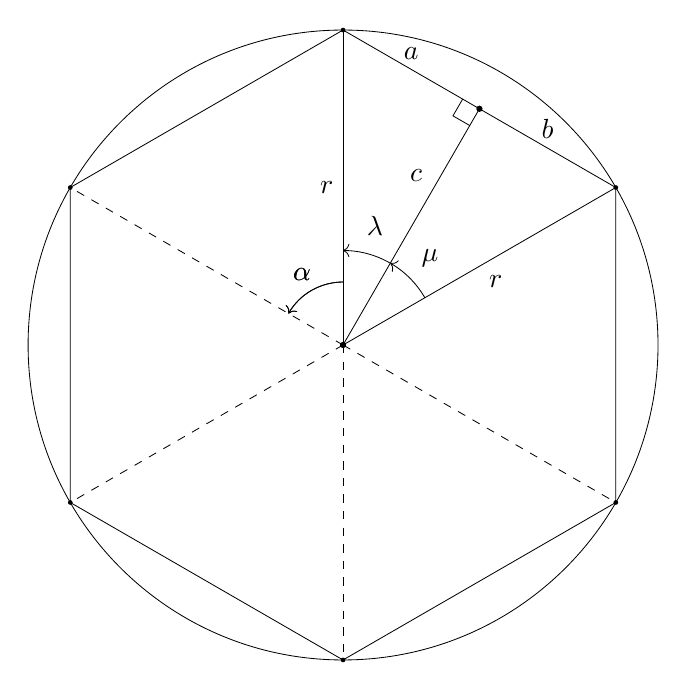
\begin{tikzpicture}[scale=1.0]

% parameters %{{{2

	% ---- length is reserved
	%\def\len{3}
	%\def\gth{3}

	% ---- angle can cause trouble
	%\def\ang{60}
	%\def\gle{60}

	\def\radius{4.0}

	\def\numsides{6}
	\def\rotation{90}

	\pgfmathtruncatemacro{\last}{\numsides}
	\pgfmathtruncatemacro{\prevlast}{\numsides-1}

% coordinates %{{{2

	\coordinate (O) at (0,0);
	\coordinate (X) at ({\rotation-360/(2*\numsides)}:\radius);

% coordinate for polygon vertices %{{{3

	\foreach \i in {1,...,\numsides} {
		\coordinate (P\i) at ({360/\numsides*(\i-1)+\rotation}:\radius);
	}

% intersections %{{{2

	\path[name path=line1] (O) -- (X);
	\path[name path=line2] (P1) -- (P\last);
	\path[name intersections={of=line1 and line2, by=A}];

% points, dots, vertices %{{{2

	\fill (O) circle (0.4mm);
	\foreach \i in {1,...,\numsides} { \fill (P\i) circle (0.3mm); }

	\fill (A) circle (0.4mm);

% segments, sides %{{{2

% polygons %{{{3

	\draw (P1) \foreach \i in {2,...,\numsides} { -- (P\i) } -- cycle;

% circles %{{{2

	\draw (O) circle (\radius);

% radiuses %{{{2

	\foreach \i in {2,...,\prevlast} { \draw[dashed] (O) -- (P\i); }

	\draw (O) -- (P1);
	\draw (O) -- (P\numsides);
	\draw (O) -- (A);

% points, dots, vertices labels %{{{2

	%\node[above] at (X) {$X$};
	%\node[above] at (A) {$A$};

% segments, sides labels %{{{2

	\node[left] at ($ (O)!0.5!(P1) $) {$r$};
	\node[below right] at ($ (O)!0.5!(P\last) $) {$r$};
	\node[above] at ($ (P1)!0.5!(A) $) {$a$};
	\node[above] at ($ (A)!0.5!(P\last) $) {$b$};
	\node[above left] at ($ (O)!0.65!(A) $) {$c$};

% segments, sides marks %{{{2

	%\tkzMarkSegments[mark=|, size=2pt](A,B)

% angles labels %{{{2

	\pic[draw, ->, "$\alpha$", angle radius=0.8cm, angle eccentricity=1.3]
	{angle = P1--O--P2};

	\pic[draw, ->, "$\lambda$", angle radius=1.2cm, angle eccentricity=1.3]
	{angle = A--O--P1};

	\pic[draw, ->, "$\mu$", angle radius=1.2cm, angle eccentricity=1.3]
	{angle = P\last--O--A};

	\pic[draw, ->, "$\alpha$", angle radius=0.8cm, angle eccentricity=1.3]
	{angle = P1--O--P2};

% right angles markers %{{{2

	\pic [draw, angle radius=7pt, angle eccentricity=1]
	{right angle = P1--A--O};

% closing %{{{2

\end{tikzpicture}
\end{document}
